\chapter{Diseases of Attitude}

In this opening lecture Jim Rohn does not give us a formal calculus so much as a disciplined sequence of maxims, comparisons, and causal sketches. The notes are therefore written in a slightly mathematical register without pretending that the source is doing economics or decision theory: we keep the lecture's progression from the normality of the negative, to the war between activity and passivity, to the visible list of diseases, and finally to the machinery of thought that feeds action and outcome.

\section{Negative Is Normal, But It Must Be Handled}

The lecture begins by removing a common resistance: we do not study the negative because it is glamorous, but because it is ordinary. The first move is therefore classificatory. Negative conditions are not an exception to life; they are part of its standing environment, like weeds in a garden.

\begin{equation}
\text{Negative} = \text{normal}, \qquad \text{Negative} \neq \text{successful}.
\end{equation}

That distinction matters. Once the negative is admitted as normal, the operative verb changes. We are not asked to adore it, and we are not allowed to deny it; we are asked to handle it. The lecture keeps returning to this practical verb because it is the hinge between passive moralizing and active self-management.

\section{The War Frame: Defaults, Oppositions, And Activity}

Rohn then enlarges the discussion into a general war frame. The point of that frame is not ornament. It lets us see that inactivity is never neutral. If good goes to sleep, something else advances.

\begin{align}
\neg \text{light} &\Rightarrow \text{darkness},\\
\neg \text{active good} &\Rightarrow \text{evil},\\
\text{sleeping democracy} &\Rightarrow \text{tyranny}.
\end{align}

These are not formal theorems; they are lecture rules. But they do real work. They tell us that the world has defaults, and the defaults are rarely on our side.

The next step is to make the war frame practical. The Old Testament ratio ``six days labor, one day rest'' is used as a small quantitative maxim. The numerical point is less about arithmetic than about rhythm.

\begin{equation}
\text{labor}:\text{rest} = 6:1.
\end{equation}

The lecturer's gloss is sharper than the familiar proverb. The hidden message is not merely that we should rest once; it is that we should not let rest become the ruling principle.

\begin{equation}
\text{enterprise} > \text{ease}, \qquad \text{activity} > \text{drift}.
\end{equation}

\paragraph{A worked heuristic.}
The internal derivation is short and worth preserving.
\begin{enumerate}
\item If the world contains an active negative, then passivity is not a stable middle state.
\item Hence the question is not whether we rest, but how much room we give the counter-force.
\item The ratio \(6:1\) is then read as a discipline of activity rather than a mere permission slip for ease.
\item From there the lecture passes naturally to the jungle metaphor: if we rest too long, the village is overtaken.
\end{enumerate}

The retirement remark belongs here as an application of the same rule. It is intentionally overstated, but its structural role is clear: too much disengagement loses the war.

\section{From War To Diagnosis: The List Begins}

Once the broad frame has been established, the lecture narrows. Rohn recaps the war and then turns to a visible list of diseases of attitude. This is where the chapter moves from general law to named diagnosis.

Before the numbered list properly begins, one transitional warning appears:

\begin{equation}
1\ \text{week of neglect} \leadsto 1\ \text{year of repair}.
\end{equation}

That equation is not on the board as such, but it is exactly how the spoken lecture compresses the cost of passivity. It also explains why the talk must now become enumerative. We are not beginning a random catalog; we are listing the mechanisms by which neglect and drift enter a life.

\begin{figure}[h]
\centering

\includegraphics[width=0.72\linewidth]{lecture_01_figure_02.png}
\caption{Chalkboard heading for the disease list. The title line is only partly legible on the board, but the screenshot preserves the lecture's turn from broad frame to named diagnosis.}
\end{figure}

The board itself is only partially readable, but the lecture makes the structure clear enough: ``Attitude Diseases,'' followed by the first item, indifference. The visible board is important precisely because it confirms that the lecture is now moving in a numbered, cumulative way.

\section{Indifference, Mildness, And Strong Feeling}

The first disease is indifference, which the lecture immediately glosses as drift and then as mildness. The point is subtle. Indifference is not spectacular failure. It is failure by low temperature.

\begin{equation}
\text{hot} \succ \text{cold} \succ \text{lukewarm}.
\end{equation}

This ranking is not a thermodynamics lesson. It is a rhetoric of commitment. Better a clear direction, even a difficult one, than the half-baked middle in which nothing decisive happens.

The lecturer then tightens the argument. If we pick a direction and go with everything we have, one of two things happens: either the path opens into opportunity, or it discloses quickly that we should be somewhere else. In that sense, commitment is epistemically useful. It reveals the truth faster than drift does.

The Saul-to-Paul story belongs here because it is not an ornamental religious detour. It functions as the lecture's living example of intensity. First the energy is misdirected; then the energy is converted. What matters for the logic of the chapter is not biography but the principle that a fully engaged person can be redirected more fruitfully than a lifeless one can be pumped up.

\section{Indecision, Doubt, Worry, And Over-Caution}

The next diseases come in a compressed cluster because they are variations on one structural fault: inward hesitation. Indecision is paralysis at the point of choice, doubt is paralysis in self-estimation, worry is paralysis in imagination, and over-caution is paralysis under risk.

The lecture's answer to self-doubt is not bravado but reversal. Turn the coin over and become a believer, beginning with belief in oneself.

\begin{equation}
\text{self-worth} \Rightarrow \text{the beginning of progress}.
\end{equation}

The transcript is garbled for a short stretch after this point, so we keep the prose close to the secure material. Worry is treated not as noble seriousness but as an expensive habit that can, with work, be given up. Over-caution is then diagnosed as the timid approach to life, and the next move is to universalize risk itself.

The lecture's central claim here is stark: life does not offer a safe region outside risk. Trying is risky; not trying has its own bill. The point is not to deny danger but to dislodge the fantasy that safety can be made fundamental.

\section{Pessimism}

Pessimism is the next disease because it gathers earlier hesitations into a settled viewpoint. The pessimist does not merely pause or worry. He has trained himself to search for the wrong side, the difficult side, the reasons something cannot be done.

\begin{figure}[h]
\centering

\includegraphics[width=0.58\linewidth]{lecture_01_figure_03.png}
\caption{Stacked chalk labels ending in pessimism. The upper labels are only partly legible, so the screenshot is kept as primary evidence.}
\end{figure}

The board at this moment is useful less as an equation than as a spatial clue. We see a narrow vertical stack of labels ending in the clearly legible word ``pessimism.'' The separator strokes are uncertain, so the clean reconstruction should be read as a cautious layout aid rather than a claim that the board contained algebra.

\begin{figure}[h]
\centering
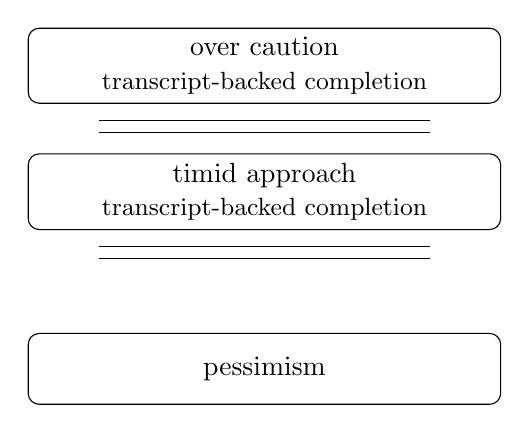
\begin{tikzpicture}
\node[draw, rounded corners, align=center, minimum width=6cm, minimum height=0.9cm] at (0,2.4) {over caution\\{\small transcript-backed completion}};
\draw (-2.1,1.7) -- (2.1,1.7);
\draw (-2.1,1.55) -- (2.1,1.55);
\node[draw, rounded corners, align=center, minimum width=6cm, minimum height=0.9cm] at (0,0.8) {timid approach\\{\small transcript-backed completion}};
\draw (-2.1,0.1) -- (2.1,0.1);
\draw (-2.1,-0.05) -- (2.1,-0.05);
\node[draw, rounded corners, align=center, minimum width=6cm, minimum height=0.9cm] at (0,-1.45) {pessimism};
\end{tikzpicture}
\caption{Cautious vertical reconstruction of the chalkboard stack. The horizontal marks are treated as separators, not equal signs.}
\end{figure}

\begin{remark}
The reconstruction above preserves only what the lecture and the board together make plausible. It should not be read as a literal transcription of every chalk stroke.
\end{remark}

\subsection{Question \& Answer}

The lecture pauses here for its cleanest explicit puzzle.

\paragraph{Question.} Why does the same measure affect two people in two different ways?

\paragraph{Answer.} Because the measure is fixed while the interpretation varies.

\begin{align}
m &= \tfrac12,\\
m &\mapsto \text{``half empty''},\\
m &\mapsto \text{``half full''}.
\end{align}

This is a small but important example. The object is the same; what changes is the reading. The lecturer's conclusion is that our lives are affected less by bare conditions than by the way we think those conditions are. Pessimism is therefore not only a mood. It is a reading protocol.

\section{The Mental Factory And The Last Disease}

Having established that interpretation matters, the lecture broadens to the machinery that forms interpretation. The mind is described as a factory, and thought as ingredient. This is the nearest thing in the lecture to a real causal model.

\begin{definition}
The \emph{mental factory} is the process by which what we repeatedly think about becomes the economic, social, and financial fabric of our lives.
\end{definition}

\begin{align}
\text{thoughts} &\rightarrow \text{ingredients},\\
\text{ingredients} &\rightarrow \text{economic/social/financial fabric}.
\end{align}

That model immediately generates a practical rule: guard the input. The examples are ordinary and vivid. Morning newspapers, trash reading, and toxic conversation are all treated as ingredient choices. Once we adopt the factory model, the logic becomes straightforward: if the inputs are poor, the output will not mysteriously become rich.

The same structure is repeated in the coffee example.

\begin{align}
\text{sugar in coffee} &\Rightarrow \text{safe},\\
\text{strychnine in coffee} &\Rightarrow \text{dead}.
\end{align}

The point is not chemistry for its own sake. The point is indifference to source. It does not matter who hands us the bad ingredient; the effect is still destructive. Hence the famous instruction to stand guard at the door of the mind.

The last disease is complaining, also named by the biblical word ``murmuring.'' The lecture is severe here because complaining is presented not as harmless ventilation but as a future-destroying habit.

\begin{equation}
5\ \text{minutes of complaining} \Rightarrow 5\ \text{minutes wasted}.
\end{equation}

The children of Israel become the final worked example. Freed from bondage, they nevertheless do not arrive at the promised land because complaint becomes their dominant mode. The logic is consistent with everything that has preceded it: a bad default, once repeatedly indulged, becomes a settled direction of life.

\section{Summary}

The lecture begins with a classification and ends with a discipline. Negative conditions are normal, but they are not to be enthroned. Because the world has defaults, inactivity yields loss; because attitude has diseases, they must be named; because interpretation shapes effect, pessimism and doubt are not trivial; and because thought becomes ingredient, the mind must be guarded. The chapter therefore closes exactly where the lecture closes: the war is on, and the practical task is to keep the good we begin from being destroyed by drift, bad input, and complaint.